\chapter{Methodology}\label{ch:methodology}

The following list provides a brief overview of our methodology which will be discussed in greater detail in the following sections:

\begin{enumerate}
    \item Preparation
    \begin{itemize}
        \item Selecting a \gls{Blockchain} network
        \item Selecting the technology stack
    \end{itemize}
    \item Development
    \begin{itemize}
        \item Versioning
        \item Agile development
        \item Interview of industry-related peers
    \end{itemize}
    \item Evaluation
    \begin{itemize}
        \item Unit tests
        \item End-to-end tests
        \item Scalability test
        \item Transaction analysis
    \end{itemize}
\end{enumerate}

\section{Preparation}\label{sec:preparation}

\subsection{Selecting a blockchain network}\label{subsec:selection-of-blockchain-network2}

To select the most feasible blockchain network, we compared the findings in \cref{sec:voting-systems} with those in \cref{subsec:comparison-of-turing-complete-blockchains}.

\subsection{Selecting the technology stack}\label{subsec:selection-of-technology-stack}

Similarly, after researching possible development tools (see \cref{sec:development-tools}), we considered a suitable technology stack.

\begin{figure}[H]
    \begin{subfigure}[b]{\textwidth}
        \centering
        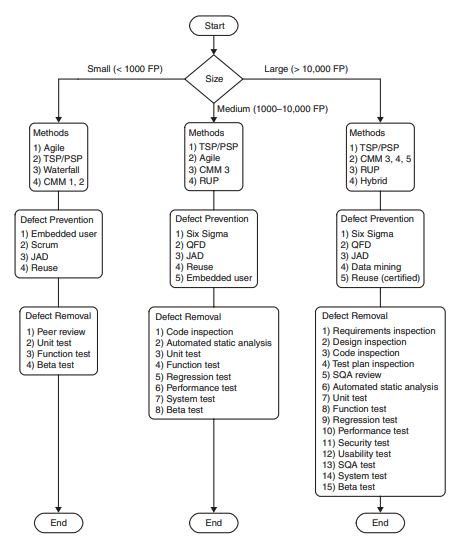
\includegraphics[width=0.7\textwidth]{jones-2010-development-methods}
        \caption[Success rates of development methods]{Success rates of development methods in relation to project size~\autocite[11]{jones_software_2010}}
        \label{fig:success-rates-development-methods}
    \end{subfigure}
    \begin{subfigure}[b]{\textwidth}
        \centering
        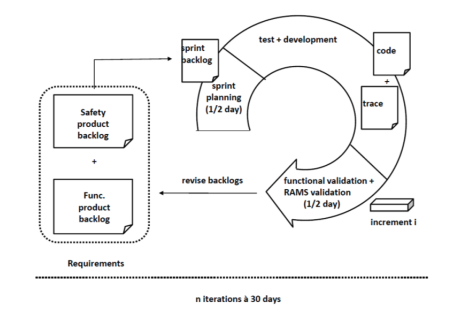
\includegraphics[scale=.8]{myklebust-2014-scrum}
        \caption[Scrum method]{Scrum method~\autocite[2]{myklebust_scrum_nodate}}
        \label{fig:scrum-method}
    \end{subfigure}
    \caption{Development methods}\label{fig:development-methods}
\end{figure}

\section{Development}\label{sec:development}

\subsection{Versioning}\label{subsec:versioning}

We used Git Workflows to version the project during development, which enabled parallel workflows depending on features, thus providing greater flexibility.
Furthermore, it enabled the analysis of code changes during our iterative processes and revision of changes.

\subsection{Agile development}\label{subsec:agile-development}

The development methods displayed in \cref{fig:success-rates-development-methods} are sorted according to their success rates.
As stated by~\textcite[10-12]{jones_software_2010}, projects with a size of less than 1000 function points are most likely to benefit from agile development methods.
The median size of function points is 53 lines of JavaScript code by~\textcite{qsm_function_2009}.
Based on these findings, we applied agile development methods during the development process as the project's size was not anticipated to grow beyond the aforementioned dimensions.

However, we departed from the recommended defect prevention methods shown in~\cref{fig:success-rates-development-methods} since embedded user reviews mainly test the application’s frontend functionality.
Instead, the same goal could be achieved by applying Scrum methods and \gls{E2E} tests.

\subsection{Personal Scrum}\label{subsec:personal-scrum}

Despite this being a one-person project with different organizational requirements than projects developed by a team, we applied scrum methods (see \cref{fig:scrum-method}) during our development process.
As \textcites{andrews_scrum_2017}{pahuja_scrum_2015} state, this meant adapting scrum methods for personal use, enabling us to establish iterative processes to track the development process, evaluate intermediate results and remove defects (see~\cref{fig:scrum-method}).

\subsection{Interview of industry-related peers}\label{subsec:interview-of-industry-member}

We collaborated with industry-related peers, who work in the \gls{Blockchain} industry, to iteratively evaluate our system, eliminate shortcomings and discuss theoretical improvements for a more sophisticated application based on our prototype.

\section{Evaluation}\label{sec:evaluation}

Our primary objective was to develop a decentralized voting system under the assumption that such a system would dramatically improve upon fundamental properties of analogous and centralized electronic systems.
We first identified objectives based on an analysis of relevant research data (see~\cref{sec:voting-systems}).
We then translated the results into software features to mirror an analogous election process and evaluated them using the methodologies discussed in the following sections.

\subsection{Unit tests}\label{subsec:unit-tests}

To ensure transactions on our \gls{SmartContract} manipulate its state in an expected manner, we employed unit tests that make use of the contract's \gls{ABI}.

\subsection{End-to-end tests}\label{subsec:end-to-end-tests}

Since code reviews are no feasible option for defect removal in a single-person project, we employed \gls{E2E} tests to evaluate the application’s intended functionality.
In contrast to unit tests, \gls{E2E} tests enabled us to evaluate entire application workflows, such as the registration or voting processes.
Most importantly, however, they provided valuable insights concerning the security of our backend services.

\subsection{Scalability test}\label{subsec:scalability-test}

As shown in~\cref{sec:voting-systems}, whether digital or analogous, voting systems must be scalable.
Therefore, we wrote scalability tests to evaluate how many voters the proposed system could handle.
In addition, a scalability test generated enough transactions on the \gls{Blockchain} to calculate the estimated network costs of our system.

\subsection{Transaction analysis}\label{subsec:transaction-analysis}

We relied on a \gls{BlockExplorer} to analyze transactions by election officials and voters committed to the blockchain network.
Consequently, we were able to evaluate transaction costs and whether voters remained anonymous (see \cref{sec:voting-systems}).
Furthermore, we tested the auditability of the election result using \glsplural{BlockExplorer}' built in features to read verified contracts' internal states.